%\documentclass[handout]{beamer}
%\documentclass{beamer}
%\documentclass[aspectratio=1610]{beamer}
\documentclass[aspectratio=1610, 10pt]{beamer}
%\documentclass[aspectratio=1610,handout, 10pt]{fbeamer}
%\NeedsTeXFormat{LaTeX2e}
%\ProvidesClass{if-beamer}[10/09/2018, v1.0.1]

\PassOptionsToPackage{svgnames}{xcolor}

\usetheme[%pageofpages=of,% String used between the current page and the
                         % total page count.
          bullet=circle,% Use circles instead of squares for bullets.
          titleline=true,% Show a line below the frame title.
          alternativetitlepage=true,% Use the fancy title page.
          titlepagelogo=logoUnicamp,% Logo for the first page.
          %watermark=watermark-unicamp,% Watermark used in every page.
          %watermarkheight=100px,% Height of the watermark.
          %watermarkheightmult=4,% The watermark image is 4 times bigger
                                % than watermarkheight.
          ]{Campinas}

\setbeamertemplate{theorems}[numbered]
\setbeamercolor{alerted text}{fg=blue!50!black}

\usepackage[square, sort]{natbib}
\bibliographystyle{plainnat} %{unsrtnat, abbrvnat, plainnat, dinat

\usepackage{epigraph}
\setlength\epigraphwidth{.9\textwidth}

\usepackage{hyperref}
\usepackage{nccmath}
\usepackage{multicol}


\usepackage[portuguese,brazil]{babel}
\usepackage{translator}
\newtranslation[to=brazil]{Example}{Exemplo}
\newtranslation[to=brazil]{Definition}{Defini\c{c}\~ao}
\newtranslation[to=brazil]{Theorem}{Teorema}
\newtranslation[to=brazil]{Corollary}{Corolário}

\usepackage[ruled,vlined,portuguese]{algorithm2e}
% \usepackage[latin1]{inputenc}
\usepackage[all]{xy}
\usepackage{times, amsmath, amsfonts, amssymb, stmaryrd} %stmaryrd}
% \usepackage{times,stmaryrd}
% \usepackage{amssymbol}
\usepackage[T1]{fontenc}
\usepackage{multirow}
\usepackage{setspace}
\usepackage{tikz} \usetikzlibrary{calc, arrows.meta, intersections, patterns, positioning, shapes.misc, fadings, through,decorations.pathreplacing}
%\usepackage[usenames,dvipsnames]{xcolor}
\usepackage{xcolor}

%\definecolor{ColorOne}{named}{MidnightBlue}
\definecolor{dandelion}{rgb}{0.94, 0.88, 0.19}
\definecolor{ColorTwo}{named}{dandelion}
%\definecolor{ColorThree}{named}{Plum}

\usepackage[portuguese]{algorithm2e}
\SetKwFor{Para}{para}{fa\c{c}a}{fim}

\usepackage{ragged2e}

\makeatletter
\renewcommand{\itemize}[1][]{%
  \beamer@ifempty{#1}{}{\def\beamer@defaultospec{#1}}%
  \ifnum \@itemdepth >2\relax\@toodeep\else
    \advance\@itemdepth\@ne
    \beamer@computepref\@itemdepth% sets \beameritemnestingprefix
    \usebeamerfont{itemize/enumerate \beameritemnestingprefix body}%
    \usebeamercolor[fg]{itemize/enumerate \beameritemnestingprefix body}%
    \usebeamertemplate{itemize/enumerate \beameritemnestingprefix body begin}%
    \list
      {\usebeamertemplate{itemize \beameritemnestingprefix item}}
      {\def\makelabel##1{%
          {%
            \hss\llap{{%
                \usebeamerfont*{itemize \beameritemnestingprefix item}%
                \usebeamercolor[fg]{itemize \beameritemnestingprefix item}##1}}%
          }%
        }%
      }
  \fi%
  \beamer@cramped%
  \justifying% NEW
  %\raggedright% ORIGINAL
  \beamer@firstlineitemizeunskip%
}
\makeatother



\newcommand{\Ll}{\pause {\color{red} \rule{\columnwidth}{1pt}}}
\newcommand{\Lp}{\pause {\color{red} \rule{\columnwidth}{1pt}}}

% Or whatever. Note that the encoding and the font should match. If T1
% does not look nice, try deleting the line with the fontenc.

\newcommand{\R}{\mathbb{R}}
\newcommand{\C}{\mathbb{C}}
\newcommand{\F}{\mathbb{F}}
\newcommand{\Z}{\mathbb{Z}}
\newcommand{\E}{\mathbb{E}}
\newcommand{\G}{\mathbb{G}}
\newcommand{\B}{\mathbb{B}}
\newcommand{\N}{\mathbb{N}}
\newcommand{\LL}{\mathbb{L}}
\newcommand{\M}{\mathbb{M}}
\newcommand{\A}{\mathbf{A}}
\newcommand{\X}{\mathbf{X}}
\newcommand{\Y}{\mathbf{Y}}
\newcommand{\FU}{\mathcal{F}(U)}
\newcommand{\FV}{\mathcal{F}(V)}
\newcommand{\ima}{\mathbf{a}}
\newcommand{\imb}{\mathbf{b}}
\newcommand{\imc}{\mathbf{c}}
\newcommand{\vets}{\mathbf{s}}
\newcommand{\impulse}{\mathbf{i}_{\mathbf{h},v}}
\newcommand{\PX}{\mathcal{P}(\mathbf{X})}

\newcommand{\vetx}{\mathbf{x}}
\newcommand{\vety}{\mathbf{y}}
\newcommand{\vetz}{\mathbf{z}}
\newcommand{\veta}{\mathbf{a}}
\newcommand{\vetb}{\mathbf{b}}
\newcommand{\vetc}{\mathbf{c}}
\newcommand{\mA}{\mathbf{A}}
\newcommand{\mB}{\mathbf{B}}
\newcommand{\mU}{\mathbf{U}}
\newcommand{\mL}{\mathbf{L}}
\newcommand{\mI}{\mathbf{I}}
\newcommand{\mD}{\mathbf{D}}

\newcommand{\bb}{\begin{equation}}
\newcommand{\ee}{\end{equation}}
\newcommand{\bbb}{\begin{eqnarray*}}
\newcommand{\eee}{\end{eqnarray*}}
\newcommand{\benu}{\begin{enumerate}}
\newcommand{\eenu}{\end{enumerate}}
\newcommand{\tr}{\mbox{tr}}

\newcommand{\vetu}{{\bf u}}
\newcommand{\vetw}{{\bf w}}
\newcommand{\vetn}{{\bf n}}
\newcommand{\tn}{\,\mathrm{t}\,}
\newcommand{\sn}{\,\mathrm{s}\,}
\newcommand{\ag}{\,\mathrm{a}\,}
\newcommand{\bpm}{\begin{bmatrix}}
\newcommand{\epm}{\end{bmatrix}}
\newcommand{\thetav}{\mbox{\boldmath$\theta$}}
\newcommand{\lambdav}{\mbox{\boldmath$\lambda$}}
\newcommand{\gammav}{\mbox{\boldmath$\gamma$}}
\newcommand{\alphav}{\mbox{\boldmath$\alpha$}}
\newcommand{\varthetav}{\mbox{\boldmath$\vartheta$}}
\newcommand{\betav}{\mbox{\boldmath$\beta$}}
\newcommand{\phiv}{\mbox{\boldmath$\phi$}}
\newcommand{\Phiv}{\mbox{\boldmath$\Phi$}}
\newcommand{\sgn}{\operatorname{sgn}}
\newcommand{\csgn}{\operatorname{csgn}}
\newcommand{\csgm}{\operatorname{csgm}}
\newcommand{\sprod}[2]{\left\langle #1, #2 \right\rangle}

\newcommand{\sen}{\operatorname{\sinhead}} \def\sinhead{sen}
\newcommand{\tg}{\operatorname{\tghead}} \def\tghead{tg}
\newcommand{\cosec}{\operatorname{\cosechead}} \def\cosechead{cosec}
\newcommand{\cotg}{\operatorname{\cotghead}} \def\cotghead{cotg}
\newcommand{\sech}{\operatorname{\sechhead}} \def\sechhead{sech}
\newcommand{\cossec}{\operatorname{\cossec}} \def\cossec{cossec}

\newcommand{\dd}[1]{\frac{d}{dx}\left[#1\right]}
\newcommand{\dt}[1]{\frac{d #1}{dt}}
\newcommand{\TFC}[3]{\left. {#1} \right|_{#2}^{#3}}
\newcommand{\Resposta}[1]{\only<2>{\alert{\textbf{Resposta: } #1}}}

\newcommand{\qeq}{\quad \mbox{e} \quad}
\newcommand{\DS}[1]{\displaystyle{#1}}

\newcommand{\bimplica}{\quad \Longleftrightarrow \quad}
\newcommand{\implica}{\quad \Longrightarrow \quad}

\newcommand{\fl}[1]{\mathtt{fl}(#1)}
\newcommand{\emach}{\varepsilon_{mach}}
\newcommand{\OO}{\mathcal{O}}

\usepackage{tcolorbox}
\newtcolorbox{mybox}[1]{colback=red!5!white,colframe=red!75!black,fonttitle=\bfseries,title=#1}
\newcommand{\tchau}{\vfill \begin{mybox}{}{\begin{center}Muito grato pela atenção!\end{center}} \end{mybox}}

\newcommand{\octave}{\texttt{GNU Octave} }
\newcommand{\python}{\texttt{python} }

\graphicspath{{Figures/}}

\setbeamerfont{caption}{size=\scriptsize}
\setbeamerfont{source}{size=\scriptsize}

\title[Regressão Descontinuada]{\huge Regressão Descontinuada}
\subtitle{\large Inferência Causal (MI628A)}

\author[Inferência Causal (MI628A)]{
    Marília Rocha \\
    Thiago Paulichen \\
    Tiago Amorim \\
    IMECC - Unicamp
}

\date{25 de Junho de 2024}

\begin{document}

\maketitle
%\onehalfspacing

\begin{frame}{}
    \epigraph{\justifying{A Regressão Descontinuada (\textit{Regression Discontinuity Design} - RDD) é utilizada  quando a atribuição do tratamento depende deterministicamente de uma covariável. Quando essa atribuição é exata, o processo de seleção é totalmente conhecido e pode ser modelado para produzir uma inferência causal não-viesada.}}{Adaptado de: \textit{Waiting for Life to Arrive} \\ \textsc{Thomas D Cook}}
\end{frame}


\begin{frame}{Sumário}
    \tableofcontents
\end{frame}


\section{Histórico}

\subsection{Linha do Tempo}


\begin{frame}{Linha do Tempo}
    \vspace{-0.3cm}
    \begin{center}
        \tikzstyle{descript} = [text = black,align=center, minimum height=1.8cm, align=center, outer sep=0pt,font = \scriptsize]
        \tikzstyle{activity} =[align=center,outer sep=1pt]

        \singlespacing
        \begin{tikzpicture}[very thick, black]
            \small

            %% Coordinates
            \coordinate (O) at (-1,0); % Origin
            \coordinate (P1) at (3,0);
            \coordinate (P2) at (4,0);
            \coordinate (P3) at (12,0);
            \coordinate (F) at (9.8,0); %End
            \coordinate (E1) at (3.4,0); %Event
            \coordinate (E2) at (1,0); %Event
            \coordinate (E3) at (4.4,0); %event
            \coordinate (E4) at (5.8,0); %event
            \coordinate (E5) at (8,0); %event
            \coordinate (E6) at (8.2,0); %event
            \coordinate (C) at (0,0); % Origin

            %% Filled regions
            \fill[color=red!25] rectangle (P1) -- (P2) -- ($(P2)+(0,0.15)$) -- ($(P1)+(0,0.15)$); % Work
            \fill[color=red!25] rectangle (P1) -- (P2) -- ($(P2)+(0,-0.15)$) -- ($(P1)+(0,-0.15)$); % Work

            %% Text inside filled regions
            \draw ($(P2)+(-2,0.5)$) node[activity,ColorTwo] {};

            %% Description
            \node[descript,text=black](D2) at ($(P2)+(-1,-2)$) {%
            	Grupo de Estudos\\
            	Universidade Northwestern\\
            	(Pré-teste, Fuzzy, não paramétrico)};

            %% Events
            \draw[<-,thick,color=black] ($(E1)+(0,0.2)$) -- ($(E1)+(0,1.5)$) node [above=0pt,align=center,black] {\scriptsize{Reinvenção e}\\[-0.1cm] \scriptsize{prova formal} \\[-0.1cm]
            \scriptsize{(Goldberger)}};
            \draw[<-,thick,color=black] ($(E2)+(0,0.2)$) -- ($(E2)+(0,1.5)$) node [above=0pt,align=center,black] {\scriptsize{Primeira publicação} \\[-0.1cm ]\scriptsize{(Thistlethwaite e} \\[-0.1cm]  \scriptsize{Campbell)}};
            \draw[<-,thick,color=black] ($(E3)+(0,0.2)$) -- ($(E3)+(0,3.3)$) node [above=0pt,align=center,black] {\scriptsize{Primeira publicação} \\[-0.1cm] \scriptsize{em Estatística (Rubin)}};
            \draw[<-,thick,color=black] ($(E4)+(0,0.2)$) -- ($(E4)+(0,1.5)$) node [above=0pt,align=center,black] {\scriptsize{Ampliação das}\\[-0.1cm] \scriptsize{aplicações} \\[-0.1cm]  \scriptsize{(Trochim)}};
            \draw[<-,thick,color=black] ($(E6)+(0,0.2)$) -- ($(E6)+(0,1.5)$) node [above=0pt,align=center,black] {\scriptsize{Apresentado como} \\[-0.1cm] \scriptsize{novo método} \\[-0.1cm] \scriptsize{(Finkelstein et.al)}};
            \draw[<-,thick,color=black] ($(E5)-(0,0.6)$) -- ($(E5)-(0,1.5)$) node [below=0pt,align=center,black] {\scriptsize{Ressurgimento do interesse} \\[-0.1cm] \scriptsize{(Política e micro-economia)}};

            %% Arrows
            \path[->,color=red!25] ($(P2)+(-0.5,0)$) edge [out=-60, in=75]  ($(D2)+(0,0.6)$);

            %% Arrow
            \draw[->] (C) -- (F);

            %% Ticks
            \foreach \x in {1,...,9}
                \draw(\x cm,3pt) -- (\x cm,-3pt);
            \foreach \x in {0.4,0.6,...,9.6}
                \draw(\x cm,2pt) -- (\x cm,-2pt);

            %% Labels
            \foreach \i \j in {1/1960,2/1965,3/1970,4/1975,5/1980,6/1985,7/1990,8/1995,9/2000}{
            	\draw (\i,0) node[below=3pt] {\j} ;
            }

        \end{tikzpicture}

        \tiny{Levantamento de \cite{cook2008waiting}}
    \end{center}
\end{frame}

\setstretch{1.25}
\setlength{\abovedisplayskip}{0.5em}
\setlength{\belowdisplayskip}{0.5em}


\subsection{Dificuldades e Ressurgimento}

\begin{frame}{Dificuldades e Ressurgimento}
\vspace{-0.4cm}
    \begin{columns}[T]
		\begin{column}{0.48\linewidth} % Left column

                \textbf{Impasses}:
                \begin{itemize}
                    \item Preconceito da comunidade estatística por um tema desenvolvido pelas ciências sociais;
                    \item Desenvolvimento inicial restrito ao grupo da Northwestern;
                    \item Papers usavam diferentes termos para RDD.
                \end{itemize}
                \textbf{Razões para o ressurgimento}:
                \begin{itemize}
                    \item Desenvolvimento por economistas renomados em diversas instituições;
                    \item Nova gama de aplicações.
                \end{itemize}

                \vspace{5pt}
                \tiny{Maiores detalhes em \cite{cook2008waiting}.}
		\end{column}
		\begin{column}{0.48\linewidth} % Right column
            \vspace{0.3cm}
            \begin{figure}
                \centering
                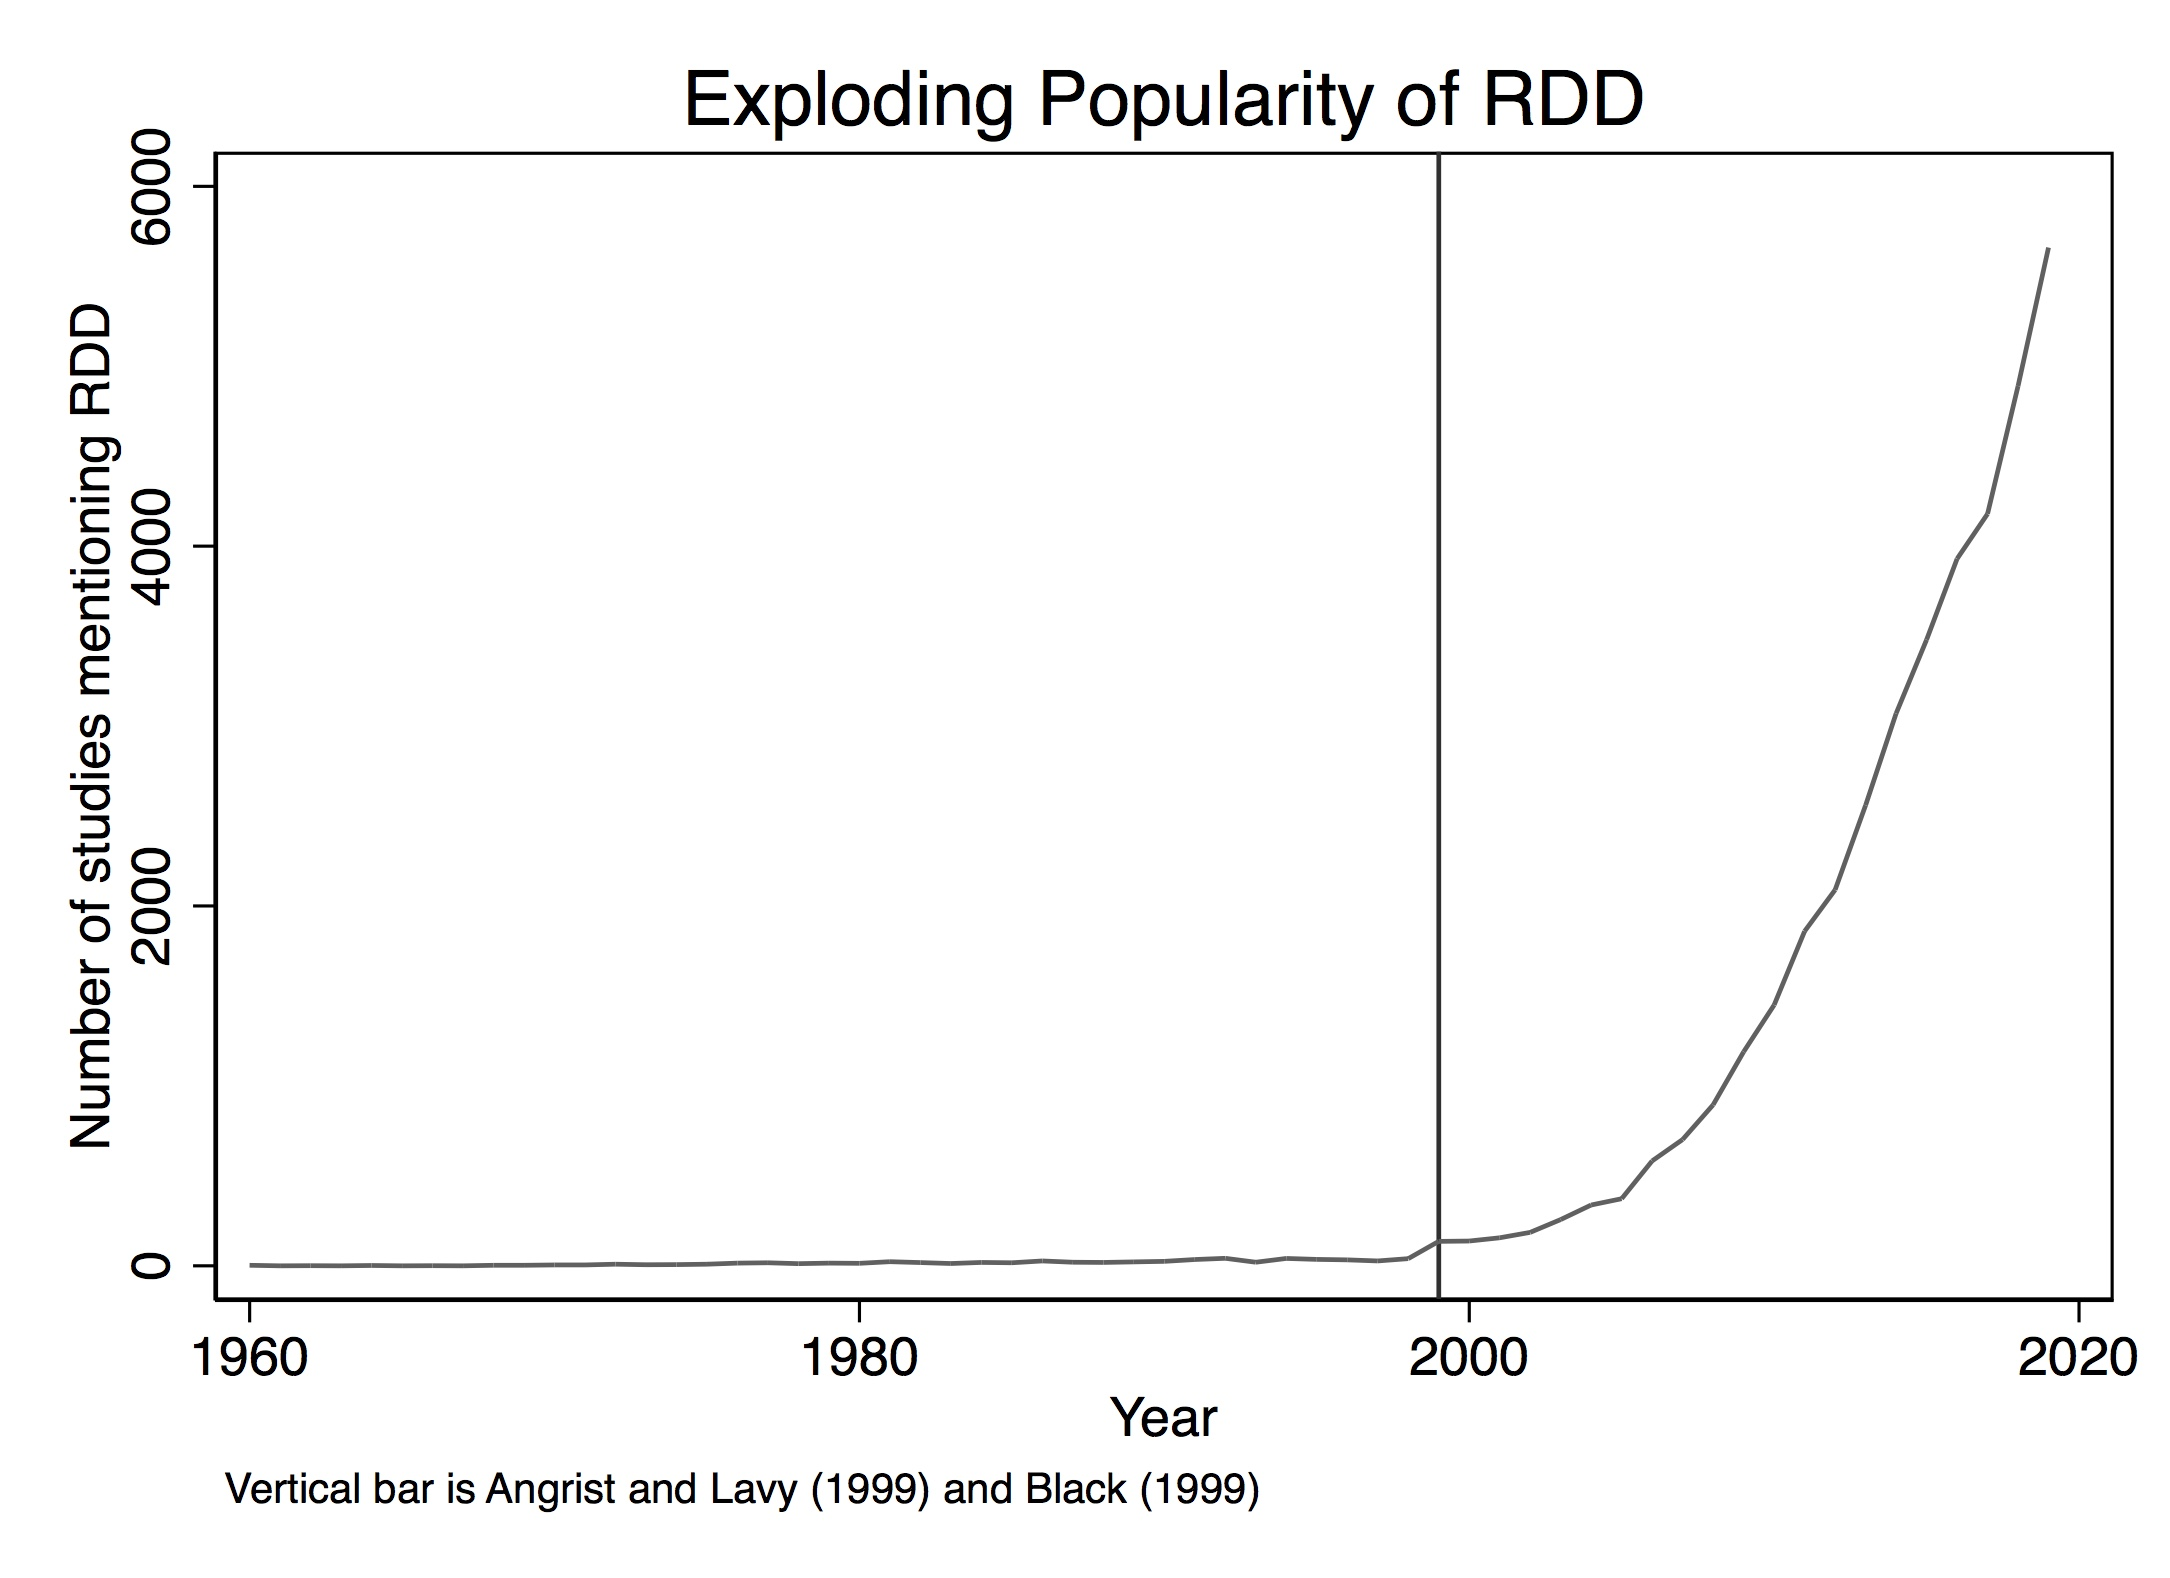
\includegraphics[width=0.95\linewidth]{fig/RDDovertime.jpg}

                \tiny{Fonte: \cite{cunningham2021causal}}
                \label{fig:enter-label}
            \end{figure}
        \end{column}
	\end{columns}
\end{frame}


\section{Regressão Descontinuada}

\begin{frame}{Descontinuidade \emph{Sharp} e \emph{Fuzzy}}
    \vspace{-0.4cm}
	\begin{columns}[T] % [T] ensures correct vertical alignment
		\begin{column}{0.48\linewidth} % Left column
         \justifying
            \textbf{Sharp}: a atribuição de tratamento segue uma regra determinista:
            \begin{equation*}
                Z_i = \begin{cases}
                    1 & \text{se } x_i \geq c \\
                    0 & \text{c.c.}
                \end{cases}
            \end{equation*}

            \vspace{0.5cm}
            \textbf{Fuzzy}: a probabilidade de atribuição de tratamento é descontínua em um ponto de corte conhecido:
            \begin{equation*}
                \mathbb{P}(Z_i=1 \mid x_i) = \begin{cases}
                    g_1(x_i) & \text{se } x_i \geq c \\
                    g_0(x_i) & \text{c.c.}
                \end{cases}
            \end{equation*}
		\end{column}
		\begin{column}{0.48\linewidth}
            \vspace{0.5cm}% Right column
            \begin{figure}
                \centering
			    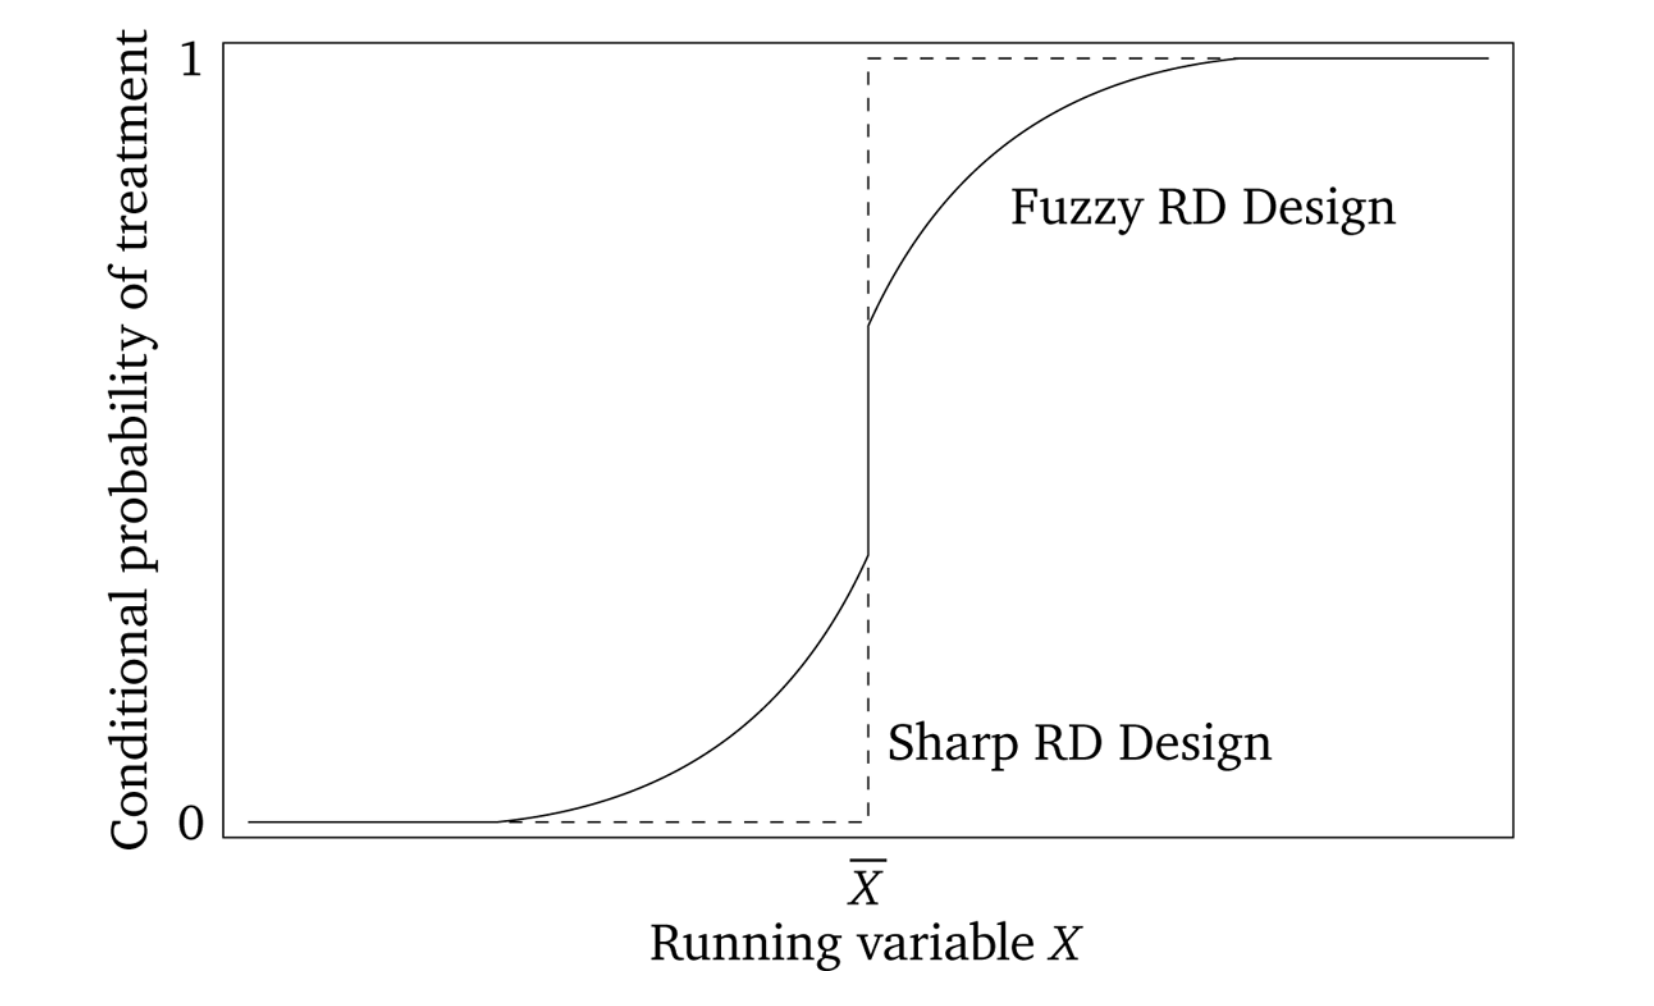
\includegraphics[width=\linewidth]{fig/SharpVsFuzzy.png}

                \tiny{Fonte: \cite{cunningham2021causal}}
            \end{figure}
        \end{column}
	\end{columns}
\end{frame}


\begin{frame}{Descontinuidade \emph{Sharp} e \emph{Fuzzy}}
    \vspace{-0.4cm}
	\begin{columns}[T] % [T] ensures correct vertical alignment
		\begin{column}{0.48\linewidth} % Left column
         \justifying
            \textbf{Sharp}: a atribuição de tratamento segue uma regra determinista:
            \begin{equation*}
                Z_i = \begin{cases}
                    1 & \text{se } x_i \geq c \\
                    0 & \text{c.c.}
                \end{cases}
            \end{equation*}

            \vspace{0.5cm}
            \textbf{Fuzzy}: a probabilidade de atribuição de tratamento é descontínua em um ponto de corte conhecido:
            \begin{equation*}
                \mathbb{P}(Z_i=1 \mid x_i) = \begin{cases}
                    g_1(x_i) & \text{se } x_i \geq c \\
                    g_0(x_i) & \text{c.c.}
                \end{cases}
            \end{equation*}
		\end{column}
		\begin{column}{0.48\linewidth}
            \textbf{Exemplos:}% Right column
            \begin{itemize}
                \item[S] Droga administrada a pacientes com uma taxa acima de certo limite.
                \item[S] Aulas de recuperação obrigatória para alunos com média abaixo de certo valor.
                \item[F] Programa da saúde suplementar oferecido à famílias que se enquadram em determinado critério de renda.
            \end{itemize}
        \end{column}
	\end{columns}
\end{frame}


\begin{frame}{Descontinuidade \emph{Sharp} e \emph{Fuzzy}}
    \begin{center}
        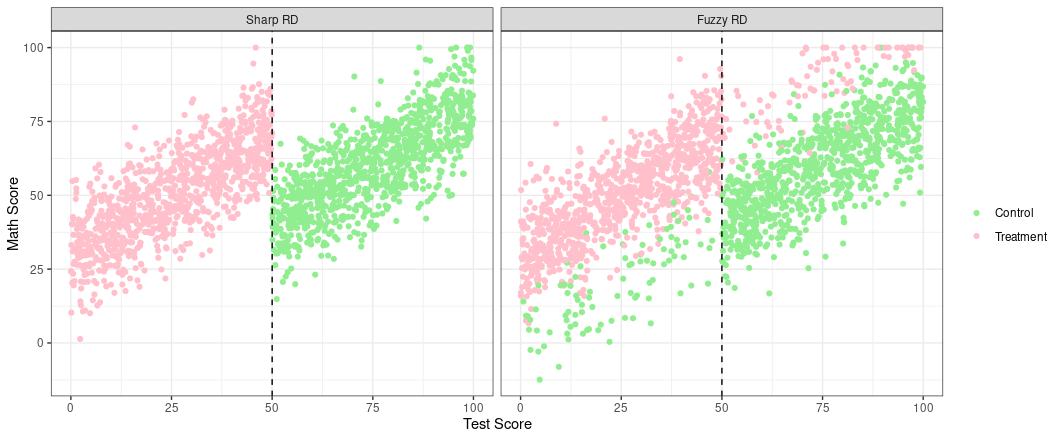
\includegraphics[width = \linewidth]{fig/FuzzySharpSimulation.png}
    \end{center}
\end{frame}


\subsection{\textit{Sharp} RD}

\begin{frame}{\textit{Sharp} RD}
    Tratamento é determinado como $Z_i = \mathbb{I}[X_i \geq c]$, onde $X_i$ é a variável de atribuição e $c$ é o ponto de corte.

    \vspace{0.3cm}
    %\pause
    \textbf{Suposições:}
    \begin{enumerate}
        \item[] \textbf{(A1)} \ $\mathbb{E}(Y_i(0) \mid X_i)$ é contínuo em $X_i = c$;
        \item[] \textbf{(A2)} \ $\mathbb{E}(Y_i(1) \mid X_i)$ é contínua em $X_i = c$;
        \item[] \textbf{(A3)} \ $\mathbb{E}(Y_i(1) - Y_i(0) \mid X_i)$ é contínua em $X_i = c$;
    \end{enumerate}

    \vspace{0.3cm}
    Um design RD foca no ponto de corte na estimação do efeito causal:
    \begin{align*}
        \tau_c := \mathbb{E}(\tau_i \mid X_i = c) = \mathbb{E}(Y_i(1) - Y_i(0) \mid X_i = c),
    \end{align*}
    e considera principalmente amostras localmente próximas ao ponto de corte.
\end{frame}

\begin{frame}{\textit{Sharp} RD}

    Dado $\varepsilon>0$ e as suposições $\textbf{(A1)}$, $\textbf{(A2)}$ e $\textbf{(A3)}$, podemos tomar os limites laterais ao longo do ponto de corte $c$, obtendo:
    \begin{align*}
        \mathbb{E}(Y_i(1) \mid X_i = c) &= \lim_{\varepsilon \rightarrow 0} \mathbb{E}(Y_i(1) \mid X_i = c + \varepsilon) \\
        &= \lim_{\varepsilon \rightarrow 0} \mathbb{E}(Y_i(1) \mid Z_i=1, X_i = c + \varepsilon) \\
        &= \lim_{\varepsilon \rightarrow 0} \mathbb{E}(Y_i \mid X_i = c + \varepsilon).
    \end{align*}
    Similarmente:
    \begin{align*}
        \mathbb{E}(Y_i(0) \mid X_i = c) &= \lim_{\varepsilon \rightarrow 0} \mathbb{E}(Y_i \mid X_i = c - \varepsilon).
    \end{align*}
    Dessa forma temos que:
    \begin{align*}
        \tau_c &=  \lim_{\varepsilon \rightarrow 0} \big[ \mathbb{E}(Y_i \mid X_i = c + \varepsilon) - \mathbb{E}(Y_i \mid X_i = c - \varepsilon) \big].
    \end{align*}
\end{frame}


\subsection{\textit{Fuzzy} RD}

\begin{frame}{\textit{Fuzzy} RD}
    \justifying
    A probabilidade condicional do tratamento $\mathbb{P}(Z_i = 1 \mid X_i)$, não pula de $0$ para $1$ no ponto de corte. $\mathbb{P}(Z_i = 1 \mid X_i)$ é descontínua em $c$ e o tamanho dessa descontinuidade está entre $0$ e $1$.
    \vspace{0.3cm}

    \textbf{Suposição adicional:}
    \begin{enumerate}
        \item[] \textbf{(A4)} $Y_i(0), Y_i(1) \perp Z_i  \mid  X_i \ $ (ignorabilidade).
    \end{enumerate}
    \vspace{0.3cm}

    Com isso, para um $\varepsilon >0$ dado, temos:
    \begin{align*}
        & \ \ \ \ \ \mathbb{E}(Y_i \mid X_i = c + \varepsilon) - \mathbb{E}(Y_i \mid X_i = c - \varepsilon) \\
        &=  \mathbb{E}(Y_i(0) + Z_i \tau_i \mid X_i = c + \varepsilon) - \mathbb{E}(Y_i(0) + Z_i \tau_i \mid X_i = c - \varepsilon) \\
      \text{\raisebox{0.2ex}{\footnotesize{\textbf{(A4)}}}} &= \mathbb{E}(Y_i(0) \mid X_i = c + \varepsilon) + \mathbb{E}(Z_i \mid X_i = c + \varepsilon) \mathbb{E}(\tau_i \mid X_i = c + \varepsilon) - \mathbb{E}(Y_i(0) \mid X_i = c - \varepsilon) \\
        & \ \ \ \ - \mathbb{E}(Z_i \mid X_i = c - \varepsilon) \mathbb{E}(\tau_i \mid X_i = c - \varepsilon).
    \end{align*}
\end{frame}

\begin{frame}{\textit{Fuzzy} RD}

 \justifying
 Fazendo o limite $\varepsilon \rightarrow 0$, segue que:
    \begin{align*}
        \lim_{\varepsilon \rightarrow 0} \big[ \mathbb{E}(Y_i \mid X_i = c + \varepsilon) - \mathbb{E}(Y_i \mid X_i = c - \varepsilon) \big] = \left(\lim_{\varepsilon \rightarrow 0} \big[ \mathbb{E}(Z_i \mid X_i = c + \varepsilon) - \mathbb{E}(Z_i \mid X_i = c - \varepsilon) \big] \right) \tau_c
    \end{align*}

    \vspace{0.15cm}
    isto é:
    \begin{align*}
        \tau_c &= \lim_{\varepsilon \rightarrow 0} \left[ \frac{\mathbb{E}(Y_i \mid X_i = c + \varepsilon) - \mathbb{E}(Y_i \mid X_i = c - \varepsilon)}{\mathbb{E}(Z_i \mid X_i = c + \varepsilon) - \mathbb{E}(Z_i \mid X_i = c - \varepsilon)} \right].
    \end{align*}

    \vspace{0.15cm}
    Observe que o caso \textit{Sharp} pode ser visto como um caso particular do \textit{Fuzzy}, uma vez que neste caso:
    \begin{align*}
        \lim_{\varepsilon \rightarrow 0} \big[ \mathbb{E}(Z_i \mid X_i = c + \varepsilon) - \mathbb{E}(Z_i \mid X_i = c - \varepsilon) \big] = 1.
    \end{align*}
\end{frame}

\subsection{Estimadores Locais}

\begin{frame}{Estimadores Locais}
\textbf{Estimador local não-paramétrico}:

\begin{align*}
   \hat{\tau}_c = \ \frac{\sum_{i:c \leq X_i < c+h} Y_i \, K\left(\frac{X_i-c}{h}\right)}{\sum_{i:c \leq X_i < c+h} K\left(\frac{X_i-c}{h} \right)} - \frac{\sum_{i:c-h < X_i < c} Y_i \, K\left(\frac{X_i-c}{h}\right)}{{\sum_{i:c-h < X_i < c} K\left(\frac{X_i-c}{h}\right)}},
\end{align*}
onde $K(u)$ é um kernel com $\int_{-1}^{1} K(u) \, du = 1$. É viesado em $\mathcal{O}(h)$.

\vspace{0.3cm}
\textbf{Estimador local linear (\emph{Sharp} RD)}:
\begin{align*}
\hat{\tau}_c = \hat{\beta}_0^+ - \hat{\beta}_0^-
\end{align*}
onde $\hat{\beta}_0^+$ e $\hat{\beta}_0^-$ vem do ajuste de $Y_i$ por mínimos quadrados:
\begin{align*}
   \textstyle  \underset{\beta^+}{\mathrm{min}} \sum_{i:c \leq X_i < c+h}(Y_i - \beta_0^+ - \beta_x^+(X_i - c))^2  \ \ \ \text{e} \ \ \
    \underset{\beta^-}{\mathrm{min}} \sum_{i:c-h < X_i < c}(Y_i - \beta_0^- - \beta_x^-(X_i - c))^2.
\end{align*}
Viés com regressão é em geral $\mathcal{O}(h^2)$.
\end{frame}



%\begin{frame}{Estimador Local}
%    \begin{columns}[T] % [T] ensures correct vertical alignment
%		\begin{column}{0.48\linewidth} % Left column
%            \textbf{Estimador local não-paramétrico}
%
%            \vspace{-0.4cm}
%            \begin{align*}
%                \hat{\tau}_c = &\frac{\sum_{i:c \leq X_i < c+h} Y_i \, K(\frac{X_i-%c}{h})}{\sum_{i:c \leq X_i < c+h} K(\frac{X_i-c}{h})} \\
%                &- \frac{\sum_{i:c-h < X_i < c} Y_i \, K(\frac{X_i-c}{h})}%{\sum_{i:c-h < X_i < c} K(\frac{X_i-c}{h})}
%            \end{align*}
%
%            onde $K(u)$ é um kernel com $\int_{-1}^{1} K(u) du = 1 $.
%
%            É enviesado em $\mathcal{O}(h)$.
%
%		\end{column}
%		\begin{column}{0.48\linewidth}
%           \textbf{Estimador local linear: \emph{Sharp} RD}
%
%            \vspace{-0.4cm}
%            \begin{equation*}
%                \hat{\tau}_c = \hat{\beta}_0^+ - \hat{\beta}_0^-
%            \end{equation*}
%
%            onde $\hat{\beta}_0^+$ e $\hat{\beta}_0^-$ vem do ajuste de $Y_i$ por mínimos quadrados:
%
%            \vspace{-0.6cm}
%            \begin{align*}
%                \min_{\beta^+} &\sum_{i:c \leq X_i < c+h}(Y_i - \beta_0^+ - %\beta_x^+(X_i - c))^2 \\
%                \min_{\beta^-} &\sum_{i:c-h < X_i < c}(Y_i - \beta_0^- - \beta_x^-%(X_i - c))^2 \\
%            \end{align*}
%
%            \vspace{-0.6cm}
%
%        \end{column}
%	\end{columns}

  %\end{frame}

%  \vspace{0.2cm}
%\cite{imbens2008regression} sugerem \textbf{fortemente} fazer regressão.
%Para descontinuidade \textit{Fuzzy} é preciso fazer ajustes de $Z_i$.

%É sugerido usar $h \propto N^{-\delta}$, com $1/5 < \delta < 2/5$ ($\delta$ é o quantil dos subgrupos).

    %Variância pode ser estimada com o estimador robusto de um \textit{Two-Stage-Least-Squares}.


\begin{frame}{Estimadores Locais}

    \begin{columns}[T] % [T] ensures correct vertical alignment
		\begin{column}{0.48\linewidth} % Left column
        \justifying
            \textbf{Estimador local linear (\emph{Fuzzy} RD)}:
            \begin{align*}
                \hat{\tau}_c = \frac{\hat{\tau}_y}{\hat{\tau}_z} = \frac{\hat{\beta}_0^+ - \hat{\beta}_0^-}{\hat{\alpha}_0^+ - \hat{\alpha}_0^-}
            \end{align*}
            onde $\hat{\beta}_0^+$ e $\hat{\beta}_0^-$ seguem fórmula para descontinuidade \emph{sharp} e $\hat{\alpha}_0^+$ e $\hat{\alpha}_0^-$ vem do ajuste de $Z_i$ por mínimos quadrados:
            \begin{align*}
               &\textstyle{ \underset{\alpha^+}{\mathrm{min}} \sum_{i:c \leq X_i < c+h}(Z_i - \alpha_0^+ - \alpha_x^+(X_i - c))^2} \\
               &\textstyle{\underset{\alpha^-}{\mathrm{min}} \sum_{i:c-h < X_i < c}(Z_i - \alpha_0^- - \alpha_x^-(X_i - c))^2 }.
            \end{align*}

            \vspace{0.1cm}
            \cite{imbens2008regression} sugerem \textbf{fortemente} fazer regressão.

            É sugerido usar $h \propto N^{-\delta}$, com $1/5 < \delta < 2/5$.

            $h$ ótimo estimado com validação cruzada.
        \end{column}
        \begin{column}{0.48\linewidth}
            \justifying
            É preciso tomar cuidado para não confundir descontinuidade com não-linearidade!

            \begin{figure}
                \centering
                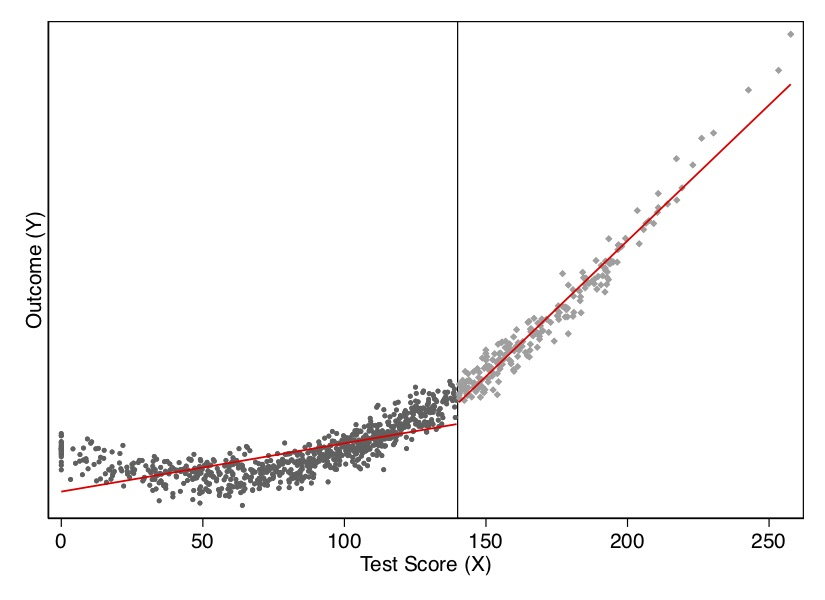
\includegraphics[width=\linewidth]{fig/NonLinear.jpg}
                \tiny{Fonte: \cite{cunningham2021causal}}
            \end{figure}

        \end{column}
	\end{columns}
\end{frame}

\begin{frame}{Estimador da Variância}
    \justifying
        Distribuição assintótica:
        \begin{align*}
            \sqrt{Nh}(\hat{\tau}-\tau) \rightarrow \mathcal{N} \left( 0,\frac{1}{\tau^2_z}V_{\tau_y}+\frac{\tau^2_y}{\tau^4_z}V_{\tau_z}-2\frac{\tau_y}{\tau^3_z}C_{\tau_y\tau_z} \right).
        \end{align*}
    Um estimador \emph{pluggin} é estimar os termos da equação acima.
    \begin{multicols}{2}[\setlength{\columnsep}{-2cm}]
    \begin{itemize}
        \item $\hat{V}_{\tau_y} = \frac{4}{\hat{f}_x(c)}(\hat{\sigma}^2_{y^+} + \hat{\sigma}^2_{y^-})$
        \item $\hat{V}_{\tau_z} = \frac{4}{\hat{f}_x(c)}(\hat{\sigma}^2_{z^+} + \hat{\sigma}^2_{z^-})$
        \item $\hat{C}_{\tau_y\tau_z} = \frac{4}{\hat{f}_x(c)}(\hat{C}_{yz^+}+\hat{C}_{yz^-})$
        \item $\hat{f}_x(x) = \frac{N_{h^+}+N_{h^-}}{2Nh}$
        \item $\hat{\sigma}^2_{y^+} = \frac{1}{N_{h^+}} \sum_{i:c \leq X_i < c+h} (Y_i - \hat{Y}(X_i))^2$
        \item $\hat{\sigma}^2_{z^+} = \frac{1}{N_{h^+}} \sum_{i:c \leq X_i < c+h} (Z_i - \hat{Z}(X_i))^2$
        \item $\hat{C}_{yz^+} = \frac{1}{N_{h^+}} \sum_{i:c \leq X_i < c+h} (Y_i - \hat{Y}(X_i))(Z_i - \hat{Z}(X_i))$
    \end{itemize}
    \end{multicols}

    Os termos \emph{negativos} tem somatório em $\{i:c-h < X_i < c\}$, e usam $N_{h^-}$.

    \vspace{0.1cm}
    Pode-se substituir pelo estimador robusto de um TSLS para RD \emph{Fuzzy} e de OLS para RD \emph{Sharp}.
\end{frame}



%\begin{frame}{Estimador da Variância}

%   \begin{aligned}
%        &\text{Distribuição assintótica:} \sqrt{Nh}(\hat{\tau}-\tau) \rightarrow \mathcal{N} \left( 0,\frac{1}{\tau^2_z}V_{\tau_y}+\frac{\tau^2_y}{\tau^4_z}V_{\tau_z}-2\frac{\tau_y}{\tau^3_z}C_{\tau_y\tau_z} \right).
%    \end{aligned}

%    \vspace{0.2cm}
%    Um estimador \emph{pluggin} é estimar os termos da equação acima.

%    \begin{columns}[T] % [T] ensures correct vertical alignment
%		\begin{column}{0.48\linewidth} % Left column
%            \begin{align*}
%                \hat{V}_{\tau_y} &= \frac{4}{\hat{f}_x(c)}(\hat{\sigma}^2_{y^+} + \hat{\sigma}^2_{y^-}) \\
%                \hat{V}_{\tau_z} &= \frac{4}{\hat{f}_x(c)}(\hat{\sigma}^2_{z^+} + \hat{\sigma}^2_{z^-}) \\
%                \hat{C}_{\tau_y\tau_z} &= \frac{4}{\hat{f}_x(c)}(\hat{C}_{yz^+}+\hat{C}_{yz^-}) \\
%                \hat{f}_x(x) &= \frac{N_{h^+}+N_{h^-}}{2Nh}
%            \end{align*}
%        \end{column}
%		\begin{column}{0.48\linewidth}
%            \begin{align*}
%                \hat{\sigma}^2_{y^+} &= \frac{1}{N_{h^+}} \sum_{i:c \leq X_i < c+h} (Y_i - \hat{Y}(X_i))^2 \\
%                \hat{\sigma}^2_{z^+} &= \frac{1}{N_{h^+}} \sum_{i:c \leq X_i < c+h} (Z_i - \hat{Z}(X_i))^2 \\
%               \hat{C}_{yz^+} &= \frac{1}{N_{h^+}} \sum_{i:c \leq X_i < c+h} (Y_i - \hat{Y}(X_i))(Z_i - \hat{Z}(X_i))
%            \end{align*}
%       \end{column}
%	\end{columns}
%    \vspace{5pt}
%    Os termos \emph{negativos} tem somatório em $\{i:c-h < X_i < c\}$, e usam $N_{h^-}$.

%    Pode substituir pelo estimador robusto de um TSLS para RD \emph{Fuzzy} e de OLS para RD \emph{Sharp}.
%\end{frame}


\subsection{Teste de Densidade de McCrary}
\begin{frame}{Teste de Densidade de McCrary}
    \justifying
    O teste de densidade de \cite{mccrary2008manipulation} ajuda a avaliar a validade dos dados.

    Avaliação envolve o uso de polinômios locais para estimar densidade.

    \begin{figure}
        \centering
        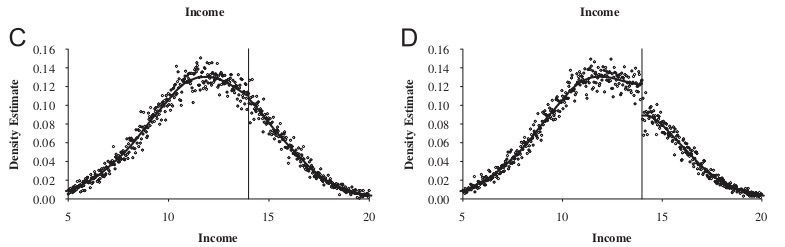
\includegraphics[width=\linewidth]{fig/McCraryDensityTest.jpg}

        \tiny{Fonte: \cite{cunningham2021causal}}
    \end{figure}
\end{frame}

\section{Exemplos}

\subsection{\emph{Toy Problem}}
\begin{frame}{\emph{Toy Problem}}
    \begin{columns}[T] % [T] ensures correct vertical alignment
		\begin{column}{0.48\linewidth} % Left column
            Função geradora dos dados:
            \begin{equation*}
                Y_i = 50 - X_i + 0.02 X_i^2 + \tau \mathbb{I}(X_i > 0) + \mathcal{N}(0,5)
            \end{equation*}

            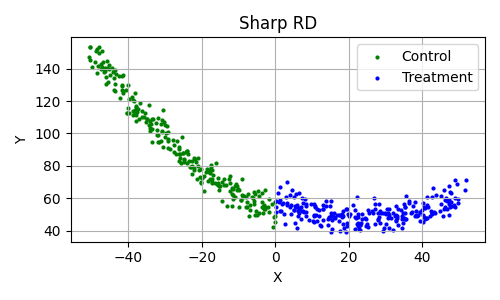
\includegraphics[width=\linewidth]{toy/SharpRD.png}
		\end{column}
		\begin{column}{0.48\linewidth}
            Avaliação da densidade de pontos.

            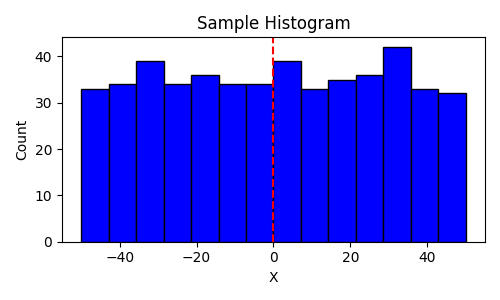
\includegraphics[width=\linewidth]{toy/SampleHistogram.png}

            Não foi encontrado código pronto em Python para cálculo da densidade local.

            Em R: \textbf{rddensity}.
        \end{column}
	\end{columns}
\end{frame}


\begin{frame}{\emph{Toy Problem}}
    \begin{columns}[T] % [T] ensures correct vertical alignment
		\begin{column}{0.48\linewidth} % Left column
            Largura da banda sugerida: \emph{h} equivalente a 20 a 40\% dos pontos de cada lado.

            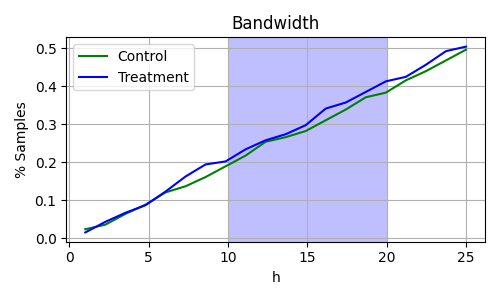
\includegraphics[width=\linewidth]{toy/Bandwidth.png}
		\end{column}
		\begin{column}{0.48\linewidth}
            \emph{Otimização} feita com validação cruzada com 50\% dos de cada lado.

            \begin{align*}
                CV(h) &= \frac{1}{N} \sum_{i}{(Y_i - \hat{Y_h}(X_i))^2} \\
                h^* &= \underset{h}{\mathrm{argmin}} \, CV(h)
            \end{align*}

            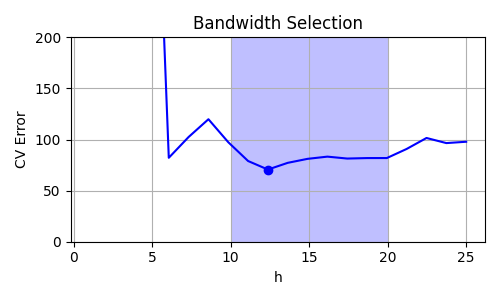
\includegraphics[width=\linewidth]{toy/BandwidthSelection.png}

        \end{column}
	\end{columns}
\end{frame}


\begin{frame}{\emph{Toy Problem}}
    \begin{columns}[T] % [T] ensures correct vertical alignment
		\begin{column}{0.48\linewidth} % Left column
            Estimador não-paramétrico local: retângulo em [c-h,c+h].

            \begin{align*}
                \hat{\tau}_c =& \frac{\sum_{i=1}^N Y_i \, \mathbb{I}(c \leq X_i < c+h)}{\sum_{i=1}^N \mathbb{I}(c \leq X_i < c+h)} \\
                &- \frac{\sum_{i=1}^N Y_i \, \mathbb{I}(c-h < X_i < c)}{\sum_{i=1}^N \mathbb{I}(c-h < X_i < c)}.
            \end{align*}

            \vspace{-0.2cm}
            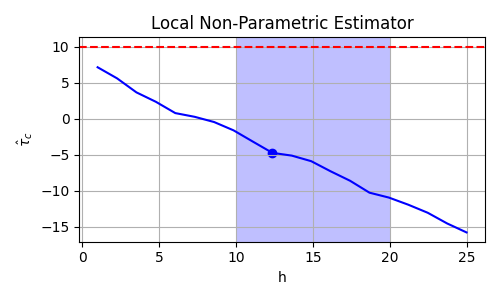
\includegraphics[width=\linewidth]{toy/LocalNonParam.png}
		\end{column}
		\begin{column}{0.48\linewidth}
            %Estimador linear local.

            \vspace{-0.3cm}
            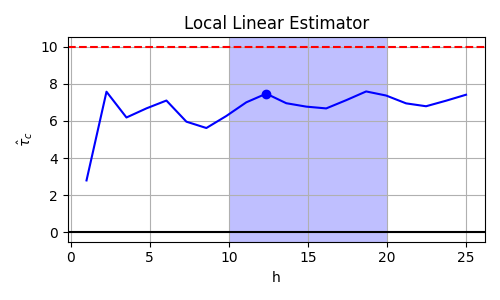
\includegraphics[width=\linewidth]{toy/LocalLinear.png}
            \vspace{-0.7cm}

            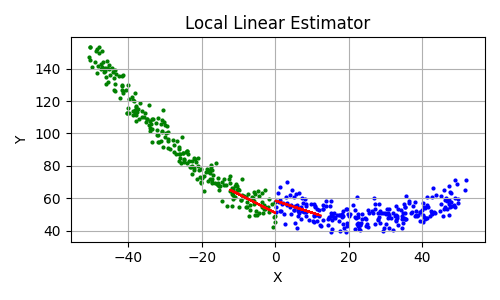
\includegraphics[width=\linewidth, trim=0cm 0cm 0cm 0.8cm, clip]{toy/LocalLinear2.png}

        \end{column}
	\end{columns}
\end{frame}


\begin{frame}{\emph{Toy Problem}}

    Para utilizar mínimos quadrados é construída uma aproximação conjunta dos dois \emph{lados}:

    \begin{equation*}
        \underset{\beta}{\mathrm{min}} \sum_{i:c-h < X_i < c+h}(Y_i - \beta_0 - \beta_x^+(X_i - c) \mathbb{I}(c \leq X_i < c+h) - \beta_x^-(X_i - c) \mathbb{I}(c - h < X_i < c) - \beta_{\tau} Z_i)^2
    \end{equation*}

    \vspace{-0.3cm}
    \centering
    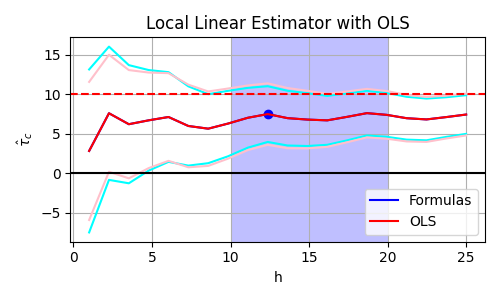
\includegraphics[width=0.7\linewidth]{toy/TauOLS.png}
\end{frame}



\subsection{\textit{Medicare}}

%\begin{frame}{\textit{Medicare}: Objetivo e Contexto}
%\begin{itemize}
%    \item \textbf{Objetivo:} Avaliar o impacto do seguro de saúde (\textit{Medicare}) na utilização de cuidados médicos. (\cite{card2008impact})
%    \item \textbf{Contexto:}
%    \begin{itemize}
%        \item \textit{Medicare} é um sistema de seguro de saúde gerido pelo governo dos Estados Unidos (EUA) e destinado às pessoas com idade igual ou maior que 65 anos. Pessoas com menos de 65 anos podem se beneficiar do programa se forem portadores de alguma deficiência ou estiverem com doenças renais graves.
%        \item Debates sobre a Lei de Cuidados Acessíveis e crescente apoio político ao programa de Seguro de Saúde para Todos (\textit{Medicare for All});
%        \item Em 2005, cerca de 20\% dos adultos não-idosos nos EUA não tinham seguro de saúde - a maioria sendo de famílias de baixa renda;
%        \item Analistas argumentam que a cobertura desigual dos seguros contribui para desigualdades na utilização de cuidados médicos e na saúde das pessoas em todos os níveis socioeconômicos.
%    \end{itemize}
%\end{itemize}
%\end{frame}

%\begin{frame}{\textit{Medicare}: Limitações e Possibilidades}
%\begin{itemize}
%    \item \textbf{Limitações:}
%    \begin{itemize}
%        \item Entre as apólices existe heterogeneidade de cobertura, o que afeta o uso;
%        \item Evidências limitadas de que melhores seguros geram impacto na saúde das pessoas - tanto a oferta como a procura de seguros dependem do estado de saúde inicial, confundindo comparações observacionais (viés de seleção).
%    \end{itemize}
%    \item \textbf{Solução:}
%    \begin{itemize}
%        \item Apenas menos de 1\% da população idosa não tem seguro (cobertura do \textit{Medicare});
%        \item Abordagem de regressão descontinuada para comparar o estado de saúde entre pessoas imediatamente antes e imediatamente após os 65 anos de idade:
%        \begin{itemize}
%            \item Mudanças no número de consultas médicas recentes e nas internações hospitalares;
%            \item Efeitos da elegibilidade ao \textit{Medicare} em diferentes subgrupos;
%            \item Quantificar até que ponto o início da elegibilidade ao \textit{Medicare} reduz ou aumenta as disparidades no uso de diferentes tipos de serviços.
%        \end{itemize}
%    \end{itemize}
%\end{itemize}
%\end{frame}




\begin{frame}{\textit{Medicare}}
        \justifying
        \textbf{Objetivo:} Avaliar o impacto do plano de saúde na utilização de cuidados médicos. (\cite{card2008impact})
        \vspace{0.3cm}

        \textbf{Limitações:} Heterogeneidade de cobertura, viés de seleção - oferta e procura dependem da saúde inicial, confundindo comparações observacionais.
        \vspace{0.3cm}

        \textbf{Solução:} Abordagem de regressão descontinuada para comparar o estado de saúde entre pessoas imediatamente antes e imediatamente após os 65 anos de idade (elegibilidade para o programa \textit{Medicare}):
        \begin{itemize}
            \item Mudanças no número de consultas médicas recentes e nas internações hospitalares;
            \item Efeitos em diferentes subgrupos;
            \item Quantificar até que ponto o início da elegibilidade ao \textit{Medicare} reduz ou aumenta as disparidades no uso de diferentes tipos de serviços.
        \end{itemize}
\end{frame}


\begin{frame}{\textit{Medicare}: Definição do modelo}
    \textbf{Modelo:}
    \begin{equation*}
        y_{ija} = X_{ija}\alpha + f_j(\alpha; \beta) + \sum_k C_{ija}^k \gamma^k + u_{ija}
    \label{model}
    \end{equation*}
    \begin{itemize}
        \item $y_{ija}$: uso de cuidados de saúde para o indivíduo $i$ no grupo socioeconômico $j$ na idade $a$;
        \item $X_{ija}$: conjunto de covariáveis (por exemplo, gênero e região);
        \item $f_j(\alpha; \beta)$: função suavizada representando o perfil de idade do resultado $y$ para o grupo $j$;
        \item $C_{ija}^k$: características da cobertura de seguro mantida pelo indivíduo;
        \item $u_{ija}$: componente de erro não observado.
    \end{itemize}
\end{frame}

\begin{frame}{\textit{Medicare}: Definição do modelo}
            \justifying
            \textbf{Problema na estimação (Cobertura do seguro é endógena):} a elegibilidade ao programa está associada a uma redução das diferenças de cobertura entre os grupos demográficos, mas há um aumento nessas diferenças quando olhamos para coberturas com mais benefícios.

            \begin{figure}
                \centering
                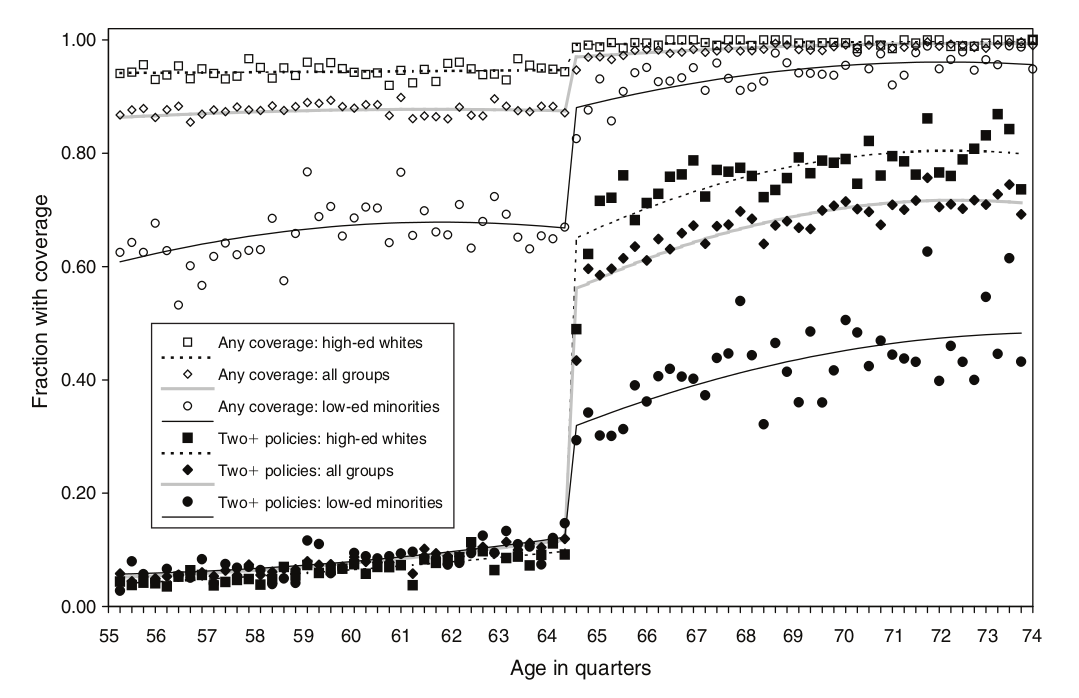
\includegraphics[scale = 0.33]{FigurasAplicacao/endogeneidade.png}
                \vspace{-0.4cm}
                \caption{Cobertura por qualquer seguro e por duas ou mais apólices, por idade e grupo demográfico.}
                \tiny{Fonte: \cite{card2008impact}}
                \label{endogeneidade}
            \end{figure}

\end{frame}



%Um problema fundamental para a estimação da equação (1) é que a cobertura do seguro é endógena. O limite de idade para elegibilidade ao Medicare aos 65 anos constitui uma fonte de variação exógena no estatuto de seguro. Para ilustrar esta afirmação, a Figura 1 mostra os perfis etários da cobertura do seguro de saúde estimados com dados do NHIS agrupado de 1999-2003, onde a idade é medida em trimestres(o exemplo está descrito abaixo e com mais detalhes no Apêndice online, disponível em http://www.aeaweb.or/articles.php?doi=10.1257/aer.98.5.2242). As taxas globais de cobertura (representadas com losangos abertos) aumentam de 85 para 96 por cento aos 65 anos. Ainda mais impressionante é o impacto da elegibilidade para o Medicare nas diferenças entre grupos socioeconomicos. Antes dos 65 anos, as minorias com menor escolaridade (negros, asiáticos e hispânicos com menos de 12 anos de escolaridade) têm taxas de cobertura 25 pontos percentuais mais baixas do que os brancos com maior escolaridade. Depois dos 65 anos a diferença cai para 10 pontos ou menos. A Figura 1 também mostra as frações de indivíduos com duas ou mais apólices de seguro. Antes dos 65 anos, a cobertura múltipla é relativamente rara. A incidência aumenta aos 65 anos, com um ganho maior para brancos com elevado nível de escolaridade, refletindo uma maior probabilidade de inscrição em políticas suplementares. Assim, a elegibilidade para o Medicare está associada a uma redução das disparidades na probabilidade de qualquer cobertura, mas a um aumento das disparidades em pelo menos um indicador da generosidade da cobertura.

\begin{frame}{\textit{Medicare}: Definição do modelo}
    \justifying
    \textbf{Solução:} Definir um modelo de probabilidade para as variáveis indicadoras $C^1_{ija}$ (qualquer cobertura) e $C^2_{ija}$ (plano com maior cobertura e com mais benefícios):
    \begin{equation*}
        C^1_{ija} = X_{ija}\beta^1_j + g_j^1(a) + D_a \pi_j^1 + \nu^1_{ija},
        \label{model_endogeneidade1}
    \end{equation*}
    \begin{equation*}
        C^2_{ija} = X_{ija}\beta^2_j + g_j^2(a) + D_a \pi_j^2 + \nu^2_{ija},
        \label{model_endogeneidade2}
    \end{equation*}
    onde $\beta^1_j$ e $\beta^2_j$ são coeficientes dos grupos socioeconômicos, $g_j^1(a)$ e $g_j^2(a)$ são perfis de idade destes grupos, e $D_a$ uma indicadora para ter 65 anos ou mais. Supondo que os perfis sejam contínuos aos 65 anos, qualquer descontinuidade em $y$ pode ser atribuída a descontinuidades no seguro.
\end{frame}

%\begin{frame}{\textit{Medicare}: Resultados}
%\begin{itemize}
    %\item \textbf{Mudanças na cobertura de seguro aos 65 anos:}
 %   Percentual de pessoas com cobertura pouco antes dos 65 anos e descontinuidades estimadas.
  %  \begin{table}
  %          \centering
  %          %\caption{Percentual de pessoas com cobertura pouco antes dos 65 anos e descontinuidades estimadas}
  %          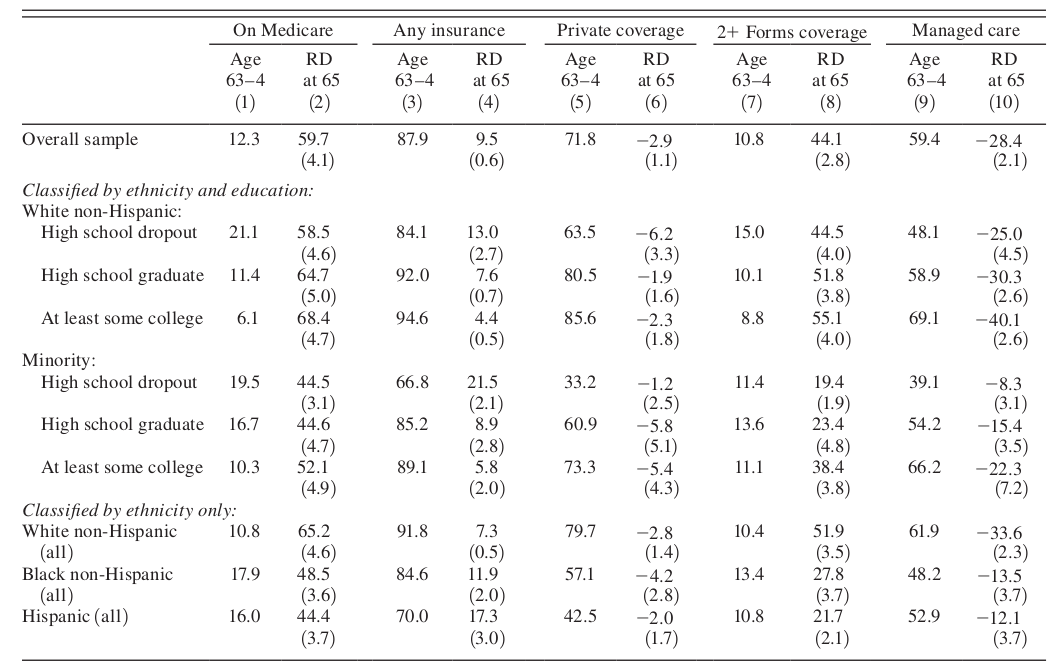
\includegraphics[scale = 0.45]{FigurasAplicacao/tabelaCobertura.png}

  %          \tiny{Fonte: \cite{card2008impact}}
  %          \label{tab_cobertura}
  %      \end{table}
%\end{itemize}
%\end{frame}

\begin{frame}{\textit{Medicare}: Resultados}
    \textbf{Mudanças na cobertura do \textit{Medicare} aos 65 anos:}
    \begin{itemize}
        \item A cobertura do aumenta em 60\% aos 65 anos;
        \item A cobertura antes dos 65 anos é maior para pessoas com escolaridade abaixo da média, e esses grupos experimentam ganhos menores aos 65 anos;
        \item Ainda existe alguma diferença na cobertura após os 65 anos, mas a diferença de 28\% entre brancos com maior escolaridade e minorias com menor escolaridade diminui para cerca de 10\%;
        \item Antes dos 65 anos, as taxas de cobertura privada variam entre 33\% para minorias com menor escolaridade e 86\% para brancos com melhor escolaridade (essas diferenças dificilmente são afetadas - a maioria dessas pessoas fazem a transição para uma combinação do \textit{Medicare} e cobertura suplementar).
    \end{itemize}
\end{frame}

\begin{frame}{\textit{Medicare}: Resultados}

\textbf{Outras mudanças aos 65 anos (aposentadoria):}
\vspace{0.1cm}

\begin{columns}[T] % [T] ensures correct vertical alignment
	\begin{column}{0.4\linewidth} % Left column
    \begin{itemize}
        \item A continuidade exige que todos os outros fatores que possam afetar o resultado tenham mudanças suaves aos 65 anos.
        \item Todos os perfis possuem comportamento suave aos 65 anos em relação à empregabilidade.
    \end{itemize}
    \end{column}
 	\begin{column}{0.6\linewidth} % Right column
        \begin{figure}
            \centering
            \vspace{-0.43cm}
            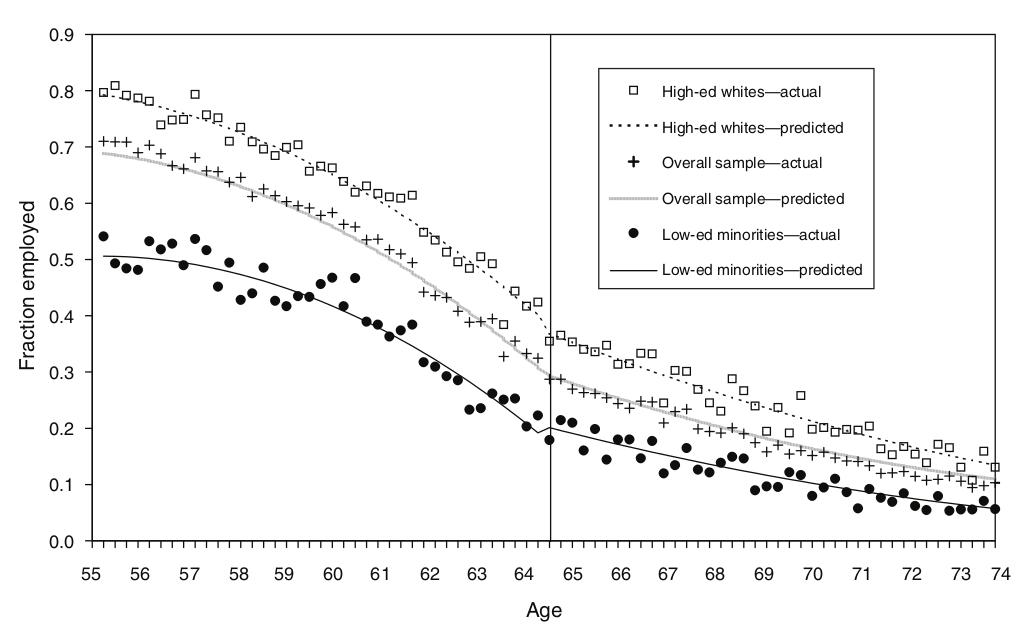
\includegraphics[scale = 0.4]{FigurasAplicacao/figuraAposentadoria.png}
            %\caption{Taxas de emprego por idade e grupo demográfico}

            \tiny{Fonte: \cite{card2008impact}}
            \label{fig_aposentadoria}
        \end{figure}
    \end{column}
\end{columns}
\end{frame}

\begin{frame}{\textit{Medicare}: Resultados}
%\begin{itemize}
    %\item \textbf{Mudanças no acesso e utilização de cuidados médicos:}
    \begin{table}
            \centering
            %\caption{Medidas de acesso aos cuidados de saúde pouco antes dos 65 anos e descontinuidades estimadas}
            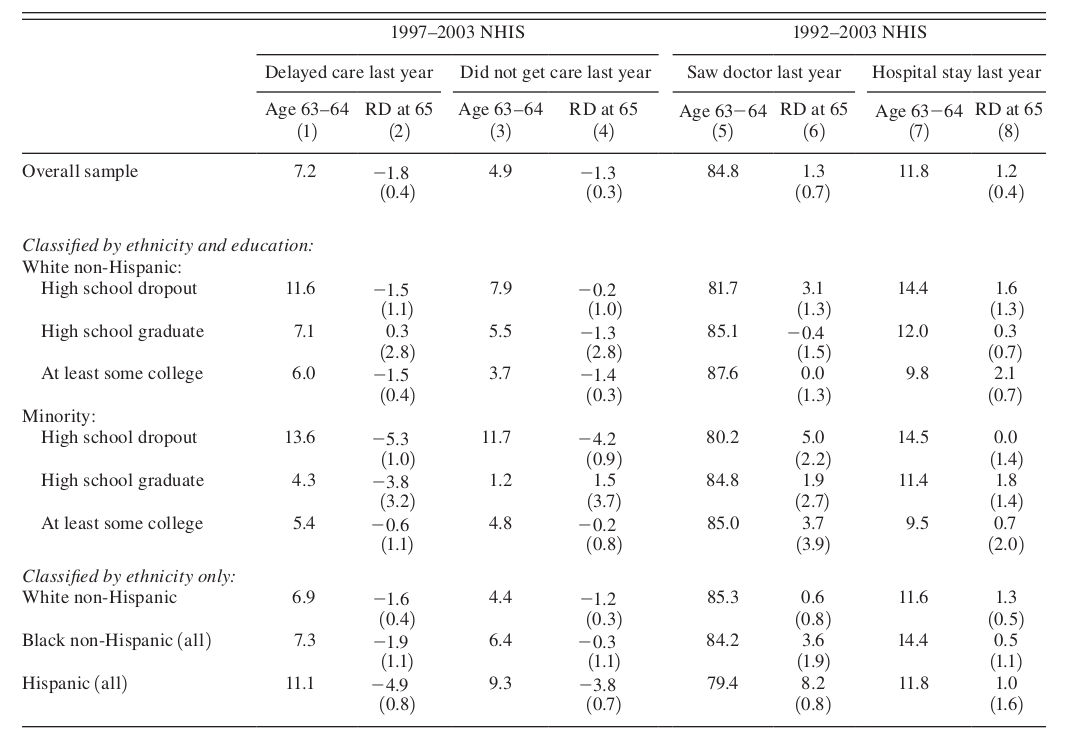
\includegraphics[scale = 0.41]{FigurasAplicacao/tabelaConsulta.png}
            \vspace{-0.3cm}
            \caption{Medidas de acesso aos cuidados de saúde pouco antes dos 65 anos e descontinuidade estimadas.}
            \tiny{Fonte: \cite{card2008impact}}
            \label{tab_consulta}
        \end{table}
%\end{itemize}
\end{frame}

\begin{frame}{\textit{Medicare}: Resultados}
    \textbf{Mudanças no acesso e utilização de cuidados médicos:}
    \begin{itemize}
        \item Cerca de 7\% das pessoas relataram atrasar os cuidados e 5\% relataram não receber cuidados, com taxas mais elevadas para as minorias com menor escolaridade e hispânicos. As estimativas implicam redução aos 65 anos em ambas as medidas;
        \item Os grupos com menor escolaridade e minoritários têm menor probabilidade de ter uma consulta de rotina, mas são mais propensos a ter passado por um período hospitalar;
        \item As estimativas sugerem que o limiar dos 65 anos está associado a um aumento nas consultas médicas de rotina, com ganhos maiores para os grupos com taxas mais baixas antes dos 65 anos;
        \item No geral, há um aumento grande nas taxas de hospitalização aos 65 anos (da ordem dos 10\%), mas os ganhos são maiores para os brancos com melhor escolaridade do que para outros grupos.
    \end{itemize}
\end{frame}

\subsection{Pacotes disponíveis}

\begin{frame}{Pacotes - Linguagem R}
    \begin{itemize}
        \item rddtools
        \item rdd
        \item rdrobust
        \item rddensity
    \end{itemize}
\end{frame}
%\begin{frame}{Aplicação - Evidências sobre o \textit{Medicare}}
%\begin{itemize}
%    \item \textbf{Resultados - Mudanças nas hospitalizações:}
%    \begin{itemize}
%        \item O aumento parece ser “permanente”, sem qualquer tendência após os 65 anos para regressar ao nível anterior, como poderia ocorrer se o salto nas admissões representasse apenas uma recuperação dos cuidados diferidos;
 %   \end{itemize}
%\end{itemize}
%\end{frame}

%\begin{frame}{Aplicação - Evidências sobre o \textit{Medicare}}
%\begin{itemize}
%    \item \textbf{Resultados - Mudanças nas hospitalizações:}
%    \begin{figure}
%            \centering
%            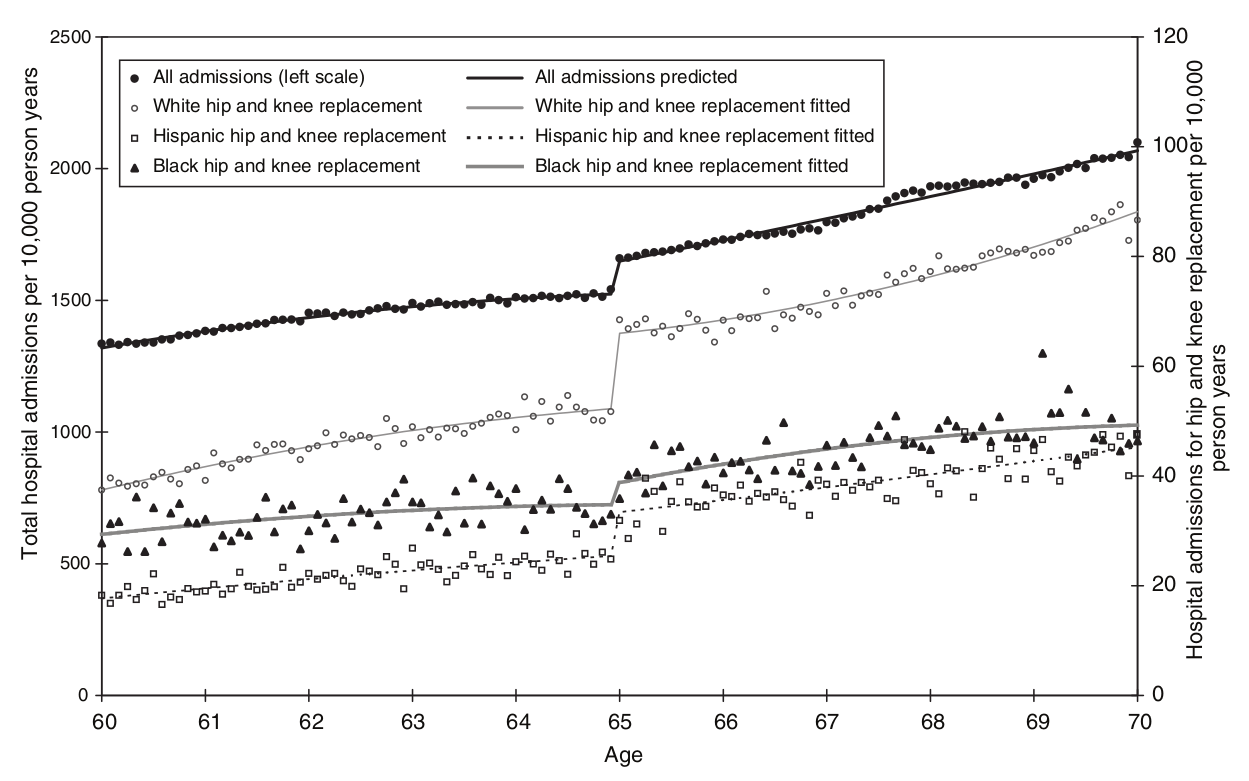
\includegraphics[scale = 0.35]{FigurasAplicacao/figuraHospital.png}
%            \caption{Taxas de internação hospitalar por raça/etnia}
%            \label{fig_hospitalizacao}
%        \end{figure}
%\end{itemize}
%\end{frame}

%\begin{frame}{Aplicação - Evidências sobre o \textit{Medicare}}
%\begin{itemize}
%    \item \textbf{Conclusão:}
%    \begin{itemize}
%        \item A elegibilidade para o \textit{Medicare} provoca um aumento acentuado na utilização de serviços de saúde, com um padrão de ganhos entre grupos que varia consoante o tipo de serviço.
%        \begin{itemize}
%            \item Para serviços de custo relativamente baixo, como consultas médicas de rotina, o início da elegibilidade para o \textit{Medicare} leva a aumentos na utilização que estão concentrados entre grupos com as taxas mais baixas de cobertura de seguro para pessoas com menos de 65 anos.
%            \item Para hospitalização para procedimentos como cirurgia de ponte de safena e prótese de quadril e joelho, os ganhos estão concentrados entre grupos que têm maior probabilidade de ter cobertura de seguro complementar após os 65 anos.
 %       \end{itemize}
 %       \item A distribuição da utilização dos serviços de saúde é impulsionada por uma interacção entre os incentivos do lado da oferta e as mudanças nas características dos seguros para diferentes grupos socioeconômicos.
 %   \end{itemize}
%\end{itemize}
%\end{frame}

%A nossa principal conclusão é que a elegibilidade para o Medicare provoca um aumento acentuado na utilização de serviços de saúde, com um padrão de ganhos entre grupos que varia consoante o tipo de serviço. Para serviços de custo relativamente baixo, como consultas médicas de rotina, o início da elegibilidade para o Medicare leva a aumentos na utilização que estão concentrados entre grupos com as taxas mais baixas de cobertura de seguro para pessoas com menos de 65 anos. incluindo hospitalização para procedimentos como cirurgia de ponte de safena e prótese de quadril e joelho – os ganhos estão concentrados entre grupos que têm maior probabilidade de ter cobertura de seguro complementar após os 65 anos. Esses padrões, juntamente com evidências de uma redistribuição de pacientes entre categorias de propriedade hospitalar, uma vez que o Medicare esteja disponível , sugerem que a distribuição dos ganhos na utilização dos serviços de saúde é impulsionada por uma interacção entre os incentivos do lado da oferta e as mudanças nas características dos seguros para diferentes grupos socioeconómicos.

\section{Referências}

\singlespacing
\begin{frame}[allowframebreaks]{Referências}
    \nocite{*}
    \bibliography{refs}
\end{frame}


\begin{frame}{}
    \begin{center}
        \Huge Perguntas?

        \begin{figure}
            
\includegraphics[width = 0.3\linewidth]{fig/qr-code.png}
        \end{figure}

    \end{center}
\end{frame}


\end{document}